\section{Human Behavior Models}


\subsection{HBM Classes}


\subsubsection{Automation Agents}
Anyone familiar with agent-based modeling is likely familiar with the behavior-desire-intent (BDI) agent architecture which has found countless applications in the automation of industry tasks such as (EXAMPLES). 
Agents of this type attempt to reproduce specific decision-making tasks reliably and predictably so that the task may be automated. 
Though extremely useful in robotics and artificial intelligence systems, these models often do not seek to represent true human-like behavior, particularly the seemingly unpredictable and irrational components. 
The goal of automation agent research is to develop an agent which can be easily told what is to be done, can express an interpretation of the given task, and can automate the task at hand reliably and accurately.

\begin{figure}[!t]
  \centering
  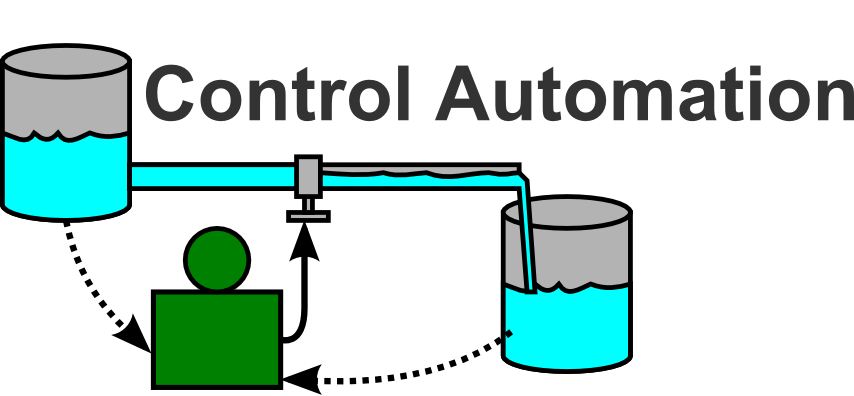
\includegraphics[width=0.5\columnwidth]{img/automationAgent}
  \caption{Human-Behavior Models designed to automate tasks such as controlling the flow of fluid between two tanks of liquid.}
  \label{automationAgent}
\end{figure}

Agents designed to replicate decision-making tasks have also found use in military strategy planning and video game AI, and through these applications have begun to incorporate variation, randomness, and ‘personality’ into the agents (\url{http://www.agent-software.com.au/applications/realistic_virtual_actors_2/}, cojack, …). 
According the terminology as defined here, this type of agent is no longer classified as an “automation agent” -- though they may be based on the BDI architecture, because the goal is no longer to simply automate a task.

\subsubsection{Emergent Behavior Studies}
Though the term agent-based modeling is often used to refer to models developed for the automation of a task or decision process (such as agents based on the BDI architecture), agent-based modeling techniques are also used to study the emergent behavior of a many-agent system. 
These emergent-behavior systems typically use a relatively simplistic agent definition and an environment with many agents to observe the behavior of the system as a whole. 
These agent models have found use in traffic simulation (Zhao 2013), MORE, and even molecular modeling (GROMACS 4.5: a high-throughput and highly parallel open source molecular simulation toolkit, Identifiability and observability analysis for experimental design in nonlinear dynamical models, bionetgen, stochsim).

\begin{figure}[!t]
  \centering
  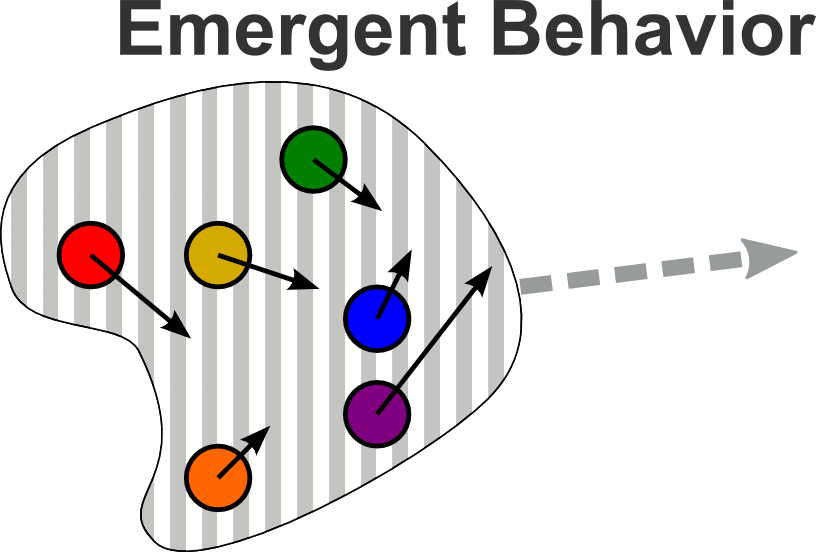
\includegraphics[width=0.5\columnwidth]{img/emergentBehavior}
  \caption{Emergent Behavior studies focus on interactions of many behavioral agents sharing one environment.}
  \label{emergentBehavior}
\end{figure}

Human behavior models developed to explore emergent behavior often neglect the intricacies of each agent’s inner workings because they are designed for efficient computation and accuracy on the level of the system rather than the individual. 

\subsubsection{Cognitive Models}
Lastly, models of human behavior are created to allow for predictive modeling of a behavioral phenomenon.
Models in this category fit the definition given by Glanz and Rimer (2005 p4): "a set of interrelated concepts, definitions and propositions that present a systematic view of events or situations by specifying relations among variables, in order to explain or predict the events or situations".
Since this type of model is useful for predicting and understanding the state of a user, formulations of theory may help overcome one of the most critical hurdles of affective computing and allow for automated intervention personalization and contextualization. 
A forecasting model can allow a human-computer interface to alter its behavior to help the user achieve a desired state. 
These models are also useful for those designing a human-computer interface or a cyber-physical system in that they can be used to estimate the ways a human may act. 

\begin{figure}[!t]
  \centering
  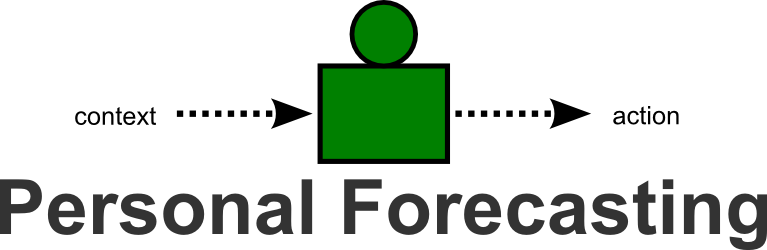
\includegraphics[width=0.5\columnwidth]{img/cognitiveHBM}
  \caption{Human behavior models which forecast human behavior focus on the translation of environmental context and internal state to future actions.}
  \label{cognitiveHBM}
\end{figure}

These models can be personalized to a subset of the population, to an individual, or may be generalizable to any healthy individual. 
Many machine learning models of human behavior and cognitive theories both fall into this category, and this type of model is of special importance to the future of automated health management systems. 
Tailored behavioral interventions, wearable sensing devices, and mHealth applications all operate based on an underlying model of human behavior which has (thus far) remained implicit in nature. 
Though all three presented classes of human behavior model may contribute to the development of the next generation of models and theories, the primary focus of this paper henceforth is on terminologies as applied to this type of human behavior model (type 3: personal forecasting).

It is important to note that behavioral forecasting models have applications outside of personalized predictions. 
Behavior forecasting models can be applied in a simulation of a population of virtual humans and compared against real data to examine the fidelity of the model or to analyze the possible effects of certain contextual stimuli. 

TODO: HBM examples /cite{Rivera}



\section{Specialist Systems UI}
* existing work on UI for “specialist systems”
